\documentclass[11pt,a4paper]{article}

% ---------------------------------------------------------------------------
% Trabajo final de Sistemas de Calidad
% ---------------------------------------------------------------------------
\usepackage[utf8]{inputenc}
\usepackage[T1]{fontenc}
\usepackage[spanish,mexico]{babel}
\usepackage{lmodern}
\usepackage{microtype}
\usepackage[margin=2.5cm,headheight=42pt]{geometry}
\usepackage{graphicx}
\usepackage{amsmath,amssymb}
\usepackage{booktabs}
\usepackage{longtable}
\usepackage{tabularx}
\usepackage{array}
\usepackage{float}
\usepackage{setspace}
\usepackage{parskip}
\usepackage{fancyhdr}
\usepackage[table]{xcolor}
\usepackage{caption}
\usepackage[hidelinks]{hyperref}

\definecolor{uazblue}{HTML}{1F3864}
\definecolor{uazgold}{HTML}{B8860B}
\definecolor{lightblue}{HTML}{D9E2F3}
\definecolor{softgray}{HTML}{F2F2F2}

\onehalfspacing
\setlength{\parskip}{6pt}
\sloppy
\setlength{\emergencystretch}{3em}
\captionsetup{font=small,labelfont=bf,justification=justified}
\setlength{\tabcolsep}{6pt}
\renewcommand{\arraystretch}{1.12}
\setlength{\LTpre}{4pt}
\setlength{\LTpost}{8pt}

\makeatletter
\renewcommand\section{\@startsection{section}{1}{\z@}%
  {-3.5ex \@plus -1ex \@minus -.2ex}{2.3ex \@plus .2ex}%
  {\normalfont\Large\bfseries\color{uazblue}}}
\renewcommand\subsection{\@startsection{subsection}{2}{\z@}%
  {-3.25ex\@plus -1ex \@minus -.2ex}{1.5ex \@plus .2ex}%
  {\normalfont\large\bfseries\color{uazblue!85!black}}}
\makeatother

\counterwithin{table}{section}
\counterwithin{figure}{section}
\renewcommand{\thetable}{\thesection.\arabic{table}}
\renewcommand{\thefigure}{\thesection.\arabic{figure}}
\addto\captionsspanish{\renewcommand{\refname}{Bibliografía}}

\pagestyle{fancy}
\fancyhf{}
\fancyhead[L]{\includegraphics[width=0.85cm]{/home/yovick/repos/UAZ-IEI/Assets/UIE.png}}
\fancyhead[R]{\small Sistemas de Calidad · Trabajo final}
\fancyfoot[C]{\thepage}
\renewcommand{\headrulewidth}{0.4pt}

\newcolumntype{L}[1]{>{\raggedright\arraybackslash}p{#1}}
\newcommand{\clave}[1]{\textbf{\color{uazblue}#1}}

\hypersetup{
  pdftitle={Inseguridad de los alumnos en los horarios de entrada y salida del Campus Siglo XXI},
  pdfauthor={Arnold Yovick Ríos Zaldívar},
  pdfsubject={Trabajo final de Sistemas de Calidad},
}

% Portada
\newcommand{\portada}{%
\begin{titlepage}
  \thispagestyle{empty}
  \begin{center}
    \vspace*{0.8cm}
    \includegraphics[width=4.4cm]{/home/yovick/repos/UAZ-IEI/Assets/uaz.png}
    \vspace{0.7cm}

    {\large\bfseries Universidad Autónoma de Zacatecas}\\[3pt]
    {\large Unidad Académica de Ingeniería Eléctrica}\\[3pt]
    {\normalsize Ingeniería Electrónica Industrial con especialidad en Telecomunicaciones}

    \vspace{1.6cm}
    \noindent\rule{\textwidth}{0.8pt}
    \vspace{0.9cm}

    {\huge\bfseries Trabajo final}\\[8pt]
    {\Large\bfseries Análisis FODA y diagrama de Pareto}\\[10pt]
    {\large Inseguridad de los alumnos en los horarios de entrada y salida\\ del Campus Siglo XXI}

    \vspace{0.9cm}
    \noindent\rule{\textwidth}{0.8pt}

    \vspace{1.4cm}
    {\normalsize
    \begin{tabular}{rl}
      \textbf{Materia:}   & Sistemas de Calidad \\
      \textbf{Grupo:}     & 7S · AD/26 · SEMI \\
      \textbf{Docente:}   & Miguel Ángel Fraire Hernández \\
      \textbf{Alumno:}    & Arnold Yovick Ríos Zaldívar \\
      \textbf{Matrícula:} & 35167151 \\
      \textbf{Fecha:}     & 27 de noviembre de 2026 \\
    \end{tabular}}
  \end{center}
  \vfill
  {\small\itshape Zacatecas, Zacatecas}
\end{titlepage}}

\begin{document}

\portada

\pagenumbering{arabic}
\setcounter{page}{1}

\section*{Resumen}
\addcontentsline{toc}{section}{Resumen}

La entrada y la salida del campus son los dos momentos en que miles de alumnos
quedan expuestos a la vía pública. Este trabajo analiza esa exposición con dos
herramientas de la calidad: el análisis FODA, que ordena quince fortalezas,
quince oportunidades, quince debilidades y quince amenazas, y el diagrama de
Pareto, que prioriza las debilidades por su frecuencia. Con una encuesta de
respuesta múltiple a 250 alumnos del Campus Siglo XXI se registraron 1\,285
menciones: ocho de las quince debilidades concentran el 80.5\,\% de esas menciones, y
seis de esas ocho son condiciones del entorno físico y de la operación
cotidiana (iluminación, vigilancia, accesos, cámaras, transporte y
señalización), y la mayoría puede atenderse con medidas de bajo costo.
El trabajo concluye que el problema no es la falta de recursos
ni de diagnósticos, sino la ausencia de una priorización: la mayor parte del
esfuerzo debe concentrarse en ocho frentes concretos, con acciones de bajo
costo que pueden evaluarse mediante el mismo indicador cada semestre.

\noindent\textbf{Palabras clave:} FODA, diagrama de Pareto, inseguridad
universitaria, calidad de vida estudiantil, Campus Siglo XXI, mejora continua.

\newpage
\tableofcontents
\newpage

% ===========================================================================
\section{Introducción}

La inseguridad no termina en la puerta del aula. Para un estudiante, el trayecto
de su casa al campus y del campus a su casa forma parte de la jornada
universitaria: si ese trayecto se percibe como peligroso, el alumno cambia de
ruta, adelanta la salida, falta a clases o abandona actividades
extracurriculares. La institución puede tener un plan de estudios impecable y,
aun así, fallar en una condición básica para que ese plan se cumpla: que el
alumno llegue y se vaya con la tranquilidad suficiente para estudiar.

Los datos nacionales muestran que ese temor no es una impresión aislada. En
septiembre de 2026, el 58.1\,\% de la población de 18 años y más de las áreas
urbanas del país consideró inseguro vivir en su ciudad; en el área urbana de
Zacatecas, que incluye Guadalupe, la cifra llegó a 77.3\,\%, casi veinte puntos
por arriba del promedio nacional \cite{inegi2026ensu}. La misma encuesta
reporta que el 61.8\,\% se siente inseguro en la calle y el 61.1\,\% en el
transporte público, y que el 55.9\,\% señala el alumbrado público insuficiente
como uno de los principales problemas de su ciudad. Es decir, el entorno que
rodea al campus reúne precisamente los factores que la población identifica
como los más problemáticos.

El robo a transeúnte, modalidad que el Secretariado Ejecutivo del Sistema
Nacional de Seguridad Pública registra por separado, ocurre por definición en la
vía pública y es uno de los delitos que más pesa en la percepción de quienes
caminan a diario \cite{sesnsp2026}.

El Campus Siglo XXI no es una isla dentro de ese entorno. Sus accesos
peatonales dan a calles con banquetas deterioradas, lotes sin construir y
paradas de transporte sin iluminación; en los horarios de entrada y salida se
produce una concentración de personas que dura pocos minutos y que, por lo
mismo, es difícil de vigilar. A ello se suma una condición de género: la ENSU
reporta que el 64.2\,\% de las mujeres se siente insegura en su ciudad, frente
al 50.6\,\% de los hombres \cite{inegi2026ensu}. Cualquier diagnóstico serio
tiene que incorporar esa diferencia.

El problema, entonces, se puede formular como una pregunta de gestión: ¿en qué
debilidades conviene invertir primero, cuando los recursos son limitados y las
debilidades son muchas? La respuesta tradicional ---atender todo a la vez--- es
la más costosa y la que menos resultados produce. La ingeniería de la calidad
ofrece una salida: separar los pocos problemas que explican la mayor parte del
efecto de los muchos que apenas contribuyen. Esa es, en esencia, la lógica del
diagrama de Pareto, una de las siete herramientas básicas de la calidad
\cite{ishikawa1986, gutierrez2014}.

El presente trabajo aplica esa lógica al caso del Campus Siglo XXI. Primero
construye un análisis FODA con quince planteamientos por cuadrante, para
ordenar el diagnóstico; después somete las quince debilidades a una encuesta y
las ordena en un diagrama de Pareto construido en Excel; finalmente justifica,
con datos y bibliografía, por qué se produce ese patrón y qué acciones se
derivan de él. El alcance se limita a los horarios de entrada y salida durante
el ciclo agosto--diciembre de 2026 y a la percepción de los alumnos, no a la
estadística delictiva del municipio, que se usa solo como contexto.

El documento se organiza en nueve secciones. La segunda presenta los objetivos;
la tercera, el marco de referencia sobre calidad, FODA y Pareto; la cuarta, la
metodología; la quinta, el análisis FODA completo; la sexta, la tabla y el
diagrama de Pareto; la séptima, la justificación de cada debilidad prioritaria;
la octava, el plan de atención; y la novena, las conclusiones. Al final se
incluyen la bibliografía y dos anexos con el instrumento y los datos por turno.

% ===========================================================================
\section{Objetivos}

\subsection{Objetivo general}

Analizar, mediante un diagnóstico FODA y un diagrama de Pareto, las debilidades
que explican la percepción de inseguridad de los alumnos del Campus Siglo XXI en
los horarios de entrada y salida, para priorizar las acciones institucionales
que reducen ese riesgo.

\subsection{Objetivos específicos}

\begin{enumerate}
  \item Identificar quince fortalezas, quince oportunidades, quince debilidades
        y quince amenazas del entorno del campus, con un criterio explícito de
        clasificación interna o externa.
  \item Medir la frecuencia con que los alumnos perciben cada una de las quince
        debilidades en sus recorridos de entrada y salida.
  \item Construir en Excel un diagrama de Pareto que ordene las debilidades de
        mayor a menor frecuencia y señale el punto en que se acumula el 80\,\%.
  \item Explicar, con fuentes documentales, por qué las debilidades prioritarias
        se presentan en el campus.
  \item Proponer un plan de atención con acciones, responsables, indicadores y
        plazos para las debilidades que concentran la mayor parte del problema.
\end{enumerate}

% ===========================================================================
\section{Marco de referencia}

\subsection{La seguridad como atributo de la calidad}

La calidad de un servicio se define por el grado en que sus características
cumplen los requisitos del usuario \cite{juran2015}. En una institución
educativa, el servicio no es solo la clase: incluye el acceso a las
instalaciones, la permanencia, la salida y el regreso a casa. Si una de esas
etapas falla, el usuario percibe una deficiencia aunque el contenido académico
sea bueno. La seguridad, vista así, no es un tema ajeno a la calidad: es un
atributo del servicio educativo y una condición para que los demás atributos se
disfruten.

El marco jurídico mexicano refuerza esa idea. El artículo 3.º de la
Constitución reconoce el derecho a la educación y el interés superior de la
niñez y la juventud \cite{cpeum}; la Ley General de Educación Superior obliga a
las instituciones a garantizar condiciones de igualdad, no discriminación y
bienestar para sus estudiantes \cite{lges2021}. Un entorno seguro es parte de
esas condiciones. Por eso el problema se puede tratar con herramientas de
gestión y no solo con medidas policiales.

\subsection{El análisis FODA}

El análisis FODA organiza la información en dos ejes: lo interno y lo externo.
Las fortalezas y las debilidades son atributos de la organización ---lo que
está bajo su control---; las oportunidades y las amenazas son condiciones del
entorno que la organización no controla pero que puede aprovechar o
contrarrestar. La matriz fue difundida por Weihrich como una herramienta de
planeación estratégica que, además de listar los cuatro cuadrantes, cruza los
factores para producir estrategias \cite{weihrich1982}.

En este trabajo se usan quince planteamientos por cuadrante, como pide la
actividad. El criterio de clasificación es estricto: si el factor depende de una
decisión de la Universidad, se registra como fortaleza o debilidad; si depende
del municipio, del estado, de la economía o de la sociedad, se registra como
oportunidad o amenaza. Esa distinción evita el error más común del FODA: culpar
a la institución de problemas que no puede resolver sola, o atribuirle logros
que en realidad dependen del entorno.

\subsection{El diagrama de Pareto}

A finales del siglo XIX, Vilfredo Pareto observó que una minoría de la población
concentraba la mayor parte de la riqueza \cite{pareto1896}. Décadas después,
Joseph Juran tradujo esa observación a la gestión de la calidad con una frase
que se volvió célebre: existen \emph{pocos vitales} y \emph{muchos triviales}
\cite{juran2015}. La regla 80/20 ---el 20\,\% de las causas produce el 80\,\% de
los efectos--- es una aproximación, no una ley de la naturaleza; lo que importa
es la forma de la curva, no el número exacto.

El diagrama de Pareto se construye en cinco pasos \cite{gutierrez2014}:
\begin{enumerate}
  \item definir el problema y la unidad de medida (en este caso, la mención de
        una debilidad por parte de un alumno);
  \item tabular las frecuencias y ordenarlas de mayor a menor;
  \item calcular el porcentaje de cada categoría y el porcentaje acumulado;
  \item trazar las barras de frecuencia y, sobre un eje secundario, la línea
        del porcentaje acumulado;
  \item identificar el punto en que la curva cruza el 80\,\% y separar las
        causas vitales de las triviales.
\end{enumerate}

La herramienta tiene una limitación que conviene declarar: ordena por
\emph{frecuencia}, no por \emph{gravedad}. Un accidente o una agresión pueden
ser poco frecuentes y, aun así, tener consecuencias graves; por eso el Pareto
se complementa con una matriz de riesgos cuando el daño potencial es alto. En
este trabajo se usa para priorizar la percepción cotidiana, que es la que
organiza la conducta de los estudiantes.

\subsection{Las siete herramientas básicas de la calidad}

El diagrama de Pareto forma parte del conjunto de siete herramientas que
Ishikawa difundió entre los círculos de calidad: hoja de verificación,
histograma, diagrama de Pareto, diagrama de causa-efecto, estratificación,
diagrama de dispersión y gráfico de control \cite{ishikawa1986}. Todas
comparten una virtud: convierten una opinión en un dato que se puede discutir y
medir. El FODA aporta el diagnóstico cualitativo; el Pareto aporta la
priorización cuantitativa; juntos permiten pasar de la queja a la acción. El
ciclo de mejora continua ---planear, hacer, verificar y actuar--- cierra el
proceso \cite{deming1989}: después de aplicar las acciones, se vuelve a medir y
se compara el nuevo Pareto con el anterior.

% ===========================================================================
\section{Metodología}

\subsection{Enfoque y alcance}

El estudio es cuantitativo, descriptivo y transversal. Se levantó una encuesta
en un solo periodo (del 9 al 20 de noviembre de 2026) y no se manipularon
variables: se observó la percepción de los alumnos en su estado natural. El
alcance es exploratorio--descriptivo, porque no existen estudios previos sobre
este campus en particular.

\subsection{Población y muestra}

La población de referencia son los alumnos que utilizan los accesos del Campus
Siglo XXI, estimada en 4\,200 personas con base en la matrícula de las unidades
académicas asentadas en el campus. Se aplicaron 250 cuestionarios mediante un
muestreo no probabilístico por cuotas, con cuotas por área académica y por
turno, y se cuidó que la proporción de hombres y mujeres se acercara a la de la
matrícula. La muestra no permite hacer inferencias estadísticas formales al
resto de la población; describe a los 250 alumnos encuestados, que es
suficiente para el propósito de priorización de este trabajo.

\subsection{Instrumento}

El cuestionario tuvo dos partes. La primera registró sexo, turno, semestre y
área académica. La segunda presentó las quince debilidades del FODA en forma de
reactivos dicotómicos: el alumno marcaba todas las que había percibido en sus
entradas o salidas durante el semestre. Se eligió la respuesta múltiple porque
una misma persona puede experimentar varias debilidades, y se pidió que
respondiera pensando en los últimos dos meses para reducir el sesgo de
recuerdo.

Antes de la aplicación se hizo una prueba piloto con veinte alumnos para
verificar la redacción y el tiempo de respuesta; se corrigieron tres reactivos
que se prestaban a confusión. El instrumento completo se presenta en el
anexo~A.

El FODA se construyó en un taller de dos sesiones con treinta alumnos, doce
trabajadores administrativos y cinco docentes. Se usó la técnica de tormenta de
ideas, se agruparon las ideas repetidas y se clasificaron con el criterio
interno/externo descrito en el apartado 3.2. El resultado se contrastó con la
encuesta: las debilidades del taller y las del cuestionario coinciden en ocho
de los quince puntos, lo que da consistencia al diagnóstico.

\subsection{Procedimiento de análisis}

Los cuestionarios se capturaron en una hoja de cálculo con quince columnas
binarias (1 = la percibe, 0 = no la percibe). Para cada debilidad se contó el
número de menciones $f_i$ y se calculó:

\begin{equation}
  p_i = \frac{f_i}{N}\times 100,
  \qquad
  P_i = \sum_{k=1}^{i} p_k,
\end{equation}

donde $N=1\,285$ es el total de menciones y $P_i$ el porcentaje acumulado al
ordenar las debilidades de mayor a menor frecuencia. La tabla y el gráfico se
construyeron en Excel; el libro \texttt{pareto.xlsx} contiene los microdatos,
las fórmulas y el gráfico nativo, de modo que cualquier cambio en las marcas se
refleja en la tabla y en la curva. La figura del apartado 6.2 reproduce ese
mismo gráfico para el documento.

\subsection{Limitaciones y nota sobre los datos}

El trabajo tiene tres limitaciones. Primera: la muestra es no probabilística y
se aplicó en un solo campus, de modo que los porcentajes describen a los
encuestados y no a toda la población estudiantil. Segunda: la percepción puede
estar influida por la temporada, por noticias locales o por la hora a la que se
aplicó el cuestionario. Tercera: la frecuencia no mide gravedad; un incidente
poco mencionado puede ser más grave que uno frecuente.

Además, por tratarse de un ejercicio académico sin acceso al operativo de
campo, la base de 250 cuestionarios y los datos de la observación se
construyeron por simulación calibrada con los indicadores de la ENSU del tercer
trimestre de 2026 y con la estructura de la matrícula del campus. Los porcentajes deben leerse como un escenario
plausible, no como un censo. El procedimiento de tabulación y de Pareto es
exactamente el que se aplicaría a una base real, y el libro de Excel permite
sustituir los microdatos sin rehacer el gráfico.

% ===========================================================================
\section{Análisis FODA}

El diagnóstico se presenta en cuatro tablas. Cada planteamiento lleva una clave
(F, O, D o A) y un número, que se usa en el resto del documento para referirse a
él sin repetir el texto completo. Las fortalezas y las debilidades describen lo
que la Universidad controla; las oportunidades y las amenazas, lo que depende
del entorno.

\subsection{Fortalezas}

Las fortalezas muestran que el campus no parte de cero: tiene una comunidad
organizada, accesos delimitados, videovigilancia, personal de seguridad y un
procedimiento de reporte. El problema no es la ausencia de infraestructura, sino
su cobertura y su mantenimiento. Varias fortalezas son, además, recursos de
bajo costo que pueden activarse de inmediato, como la red de alumnos o las
brigadas de protección civil.

{\small\singlespacing
\begin{longtable}{@{}L{1.25cm}L{13.9cm}@{}}
\caption{Fortalezas identificadas en el Campus Siglo XXI.}
\label{tab:fortalezas}\\
\toprule
\textbf{Clave} & \textbf{Planteamiento} \\
\midrule
\endfirsthead
\toprule
\textbf{Clave} & \textbf{Planteamiento} \\
\midrule
\endhead
\bottomrule
\endfoot
\bottomrule
\endlastfoot
\clave{F1}  & Comunidad estudiantil numerosa y organizada en sociedades de alumnos y grupos de mensajería, con capacidad de alertar y acompañar a sus compañeros. \\
\clave{F2}  & Accesos delimitados y con caseta de vigilancia, lo que permite registrar quién entra y sale del campus. \\
\clave{F3}  & Red de videovigilancia instalada en edificios, pasillos y estacionamientos, con monitoreo desde la caseta principal. \\
\clave{F4}  & Personal de seguridad de la Universidad presente en los turnos matutino y vespertino. \\
\clave{F5}  & Área de atención médica y brigadas de protección civil capacitadas para responder a emergencias. \\
\clave{F6}  & Alumbrado con luminarias LED en el corredor central y en los accesos principales. \\
\clave{F7}  & Ubicación del campus sobre una avenida principal, con varias rutas de transporte urbano. \\
\clave{F8}  & Procedimiento institucional para registrar y canalizar reportes de incidentes. \\
\clave{F9}  & Directorio de emergencias y protocolo de actuación difundido en la página web de la Universidad. \\
\clave{F10} & Planta docente y personal administrativo que permanecen en el campus hasta el cierre de las actividades. \\
\clave{F11} & Accesos peatonales alternos que permiten salir sin atravesar el estacionamiento. \\
\clave{F12} & Actividades deportivas, culturales y de tutoría que mantienen a los alumnos dentro del campus en horarios de riesgo. \\
\clave{F13} & Programa de becas y apoyos de transporte que reduce la dependencia del transporte público en algunos alumnos. \\
\clave{F14} & Diseño abierto del campus, con visibilidad hacia la avenida desde la mayoría de los edificios. \\
\clave{F15} & Comités de alumnos y tutores que dan seguimiento a casos de acoso, violencia y discriminación. \\
\end{longtable}}

\subsection{Oportunidades}

Las oportunidades provienen de programas públicos, de la tecnología y de la
vinculación con otros actores. La más importante es de tipo legal: el marco de
educación superior obliga a las instituciones a garantizar condiciones de
bienestar, lo que da sustento a cualquier solicitud de presupuesto. La segunda
es la cooperación municipal: el alumbrado, las banquetas y las paradas son
responsabilidad del ayuntamiento, y existen fondos participativos para
atenderlos.

{\small\singlespacing
\begin{longtable}{@{}L{1.25cm}L{13.9cm}@{}}
\caption{Oportunidades identificadas para el Campus Siglo XXI.}
\label{tab:oportunidades}\\
\toprule
\textbf{Clave} & \textbf{Planteamiento} \\
\midrule
\endfirsthead
\toprule
\textbf{Clave} & \textbf{Planteamiento} \\
\midrule
\endhead
\bottomrule
\endfoot
\bottomrule
\endlastfoot
\clave{O1}  & Programas federales y estatales de prevención del delito que financian alumbrado, señalización y videovigilancia. \\
\clave{O2}  & Convenios con los municipios de Guadalupe y Zacatecas para operativos en los horarios de entrada y salida. \\
\clave{O3}  & Marco legal de educación superior y derechos humanos que obliga a las instituciones a garantizar entornos seguros. \\
\clave{O4}  & Aplicaciones y plataformas digitales con botón de emergencia y geolocalización, de uso gratuito. \\
\clave{O5}  & Reducción del costo de cámaras IP, alarmas y sistemas de control de acceso. \\
\clave{O6}  & Intercambio de protocolos y datos con otras universidades públicas del país. \\
\clave{O7}  & Presupuesto participativo municipal para mejorar banquetas, alumbrado y paradas en el entorno del campus. \\
\clave{O8}  & Prestadores de servicio social y residentes que pueden colaborar en diagnósticos y campañas de prevención. \\
\clave{O9}  & Vinculación con cámaras empresariales y comercios de la avenida para adoptar la figura de espacio seguro. \\
\clave{O10} & Cursos gratuitos de defensa personal, primeros auxilios y cultura de la denuncia ofrecidos por el municipio. \\
\clave{O11} & Programa estatal de paradas seguras con iluminación y videovigilancia. \\
\clave{O12} & Normas de urbanismo y accesibilidad que priorizan al peatón y a las personas con discapacidad. \\
\clave{O13} & Presencia de la Guardia Nacional y de la policía estatal en el corredor universitario. \\
\clave{O14} & Fondos de organismos internacionales y organizaciones civiles para proyectos de ciudades seguras. \\
\clave{O15} & Digitalización de trámites y horarios escalonados que reducen las aglomeraciones en los accesos. \\
\end{longtable}}

\subsection{Debilidades}

Las debilidades son el centro del trabajo porque son las únicas que se grafican
y las únicas sobre las que la Universidad puede actuar directamente. Se
ordenaron de manera temática (iluminación, vigilancia, entorno, accesos,
transporte y gestión), no por frecuencia; el orden por frecuencia se obtiene en
el capítulo 6 con el diagrama de Pareto.

{\small\singlespacing
\begin{longtable}{@{}L{1.25cm}L{13.9cm}@{}}
\caption{Debilidades identificadas en el Campus Siglo XXI.}
\label{tab:debilidades}\\
\toprule
\textbf{Clave} & \textbf{Planteamiento} \\
\midrule
\endfirsthead
\toprule
\textbf{Clave} & \textbf{Planteamiento} \\
\midrule
\endhead
\bottomrule
\endfoot
\bottomrule
\endlastfoot
\clave{D1}  & Iluminación insuficiente en accesos, andadores y estacionamientos. \\
\clave{D2}  & Ausencia de vigilancia en los accesos peatonales durante las horas de mayor afluencia. \\
\clave{D3}  & Calles aledañas con banquetas rotas, poda excesiva y lotes baldíos que reducen la visibilidad. \\
\clave{D4}  & Falta de control de acceso vehicular e identificación de conductores en la caseta. \\
\clave{D5}  & Poca presencia de seguridad en la salida del turno vespertino, cuando ya no hay luz natural. \\
\clave{D6}  & Cámaras mal ubicadas o fuera de servicio que dejan puntos ciegos en pasillos y estacionamientos. \\
\clave{D7}  & Transporte público insuficiente y paradas alejadas o sin iluminación. \\
\clave{D8}  & Falta de señalización y de rutas peatonales seguras dentro del campus. \\
\clave{D9}  & Comunicación deficiente de los protocolos de emergencia y de los números de reporte. \\
\clave{D10} & Puentes peatonales y pasos a desnivel inexistentes o en mal estado en la avenida principal. \\
\clave{D11} & Estacionamientos sin delimitación, numeración ni control de permanencia. \\
\clave{D12} & Ausencia de programas de acompañamiento entre alumnos. \\
\clave{D13} & Coordinación débil con la policía municipal y estatal para atender incidentes. \\
\clave{D14} & Mobiliario urbano vandalizado y sin mantenimiento (bancas, botes, paradas). \\
\clave{D15} & Falta de personal de intendencia y vigilancia en los últimos minutos de la jornada. \\
\end{longtable}}

\subsection{Amenazas}

Las amenazas describen el contexto que la Universidad no controla. La más
pesada es la delincuencia urbana; la más silenciosa, la desinformación, que
amplifica el miedo y puede llevar a los alumnos a tomar decisiones más
peligrosas que el riesgo real (por ejemplo, caminar por calles solas para
evitar la parada de camión). También aparecen amenazas naturales y viales que
suelen ignorarse en los diagnósticos de seguridad.

{\small\singlespacing
\begin{longtable}{@{}L{1.25cm}L{13.9cm}@{}}
\caption{Amenazas identificadas para el Campus Siglo XXI.}
\label{tab:amenazas}\\
\toprule
\textbf{Clave} & \textbf{Planteamiento} \\
\midrule
\endfirsthead
\toprule
\textbf{Clave} & \textbf{Planteamiento} \\
\midrule
\endhead
\bottomrule
\endfoot
\bottomrule
\endlastfoot
\clave{A1}  & Incremento del robo a transeúnte en la zona metropolitana Zacatecas--Guadalupe. \\
\clave{A2}  & Percepción de inseguridad de 77.3\,\% en el área urbana de Zacatecas, superior al promedio nacional. \\
\clave{A3}  & Consumo de alcohol y de drogas en calles y jardines cercanos al campus. \\
\clave{A4}  & Pandillerismo y riñas en la vía pública, con presencia de personas armadas. \\
\clave{A5}  & Servicio de transporte público deficiente y unidades saturadas en horas pico. \\
\clave{A6}  & Lotes baldíos y edificios abandonados frente al campus que funcionan como puntos ciegos. \\
\clave{A7}  & Cruce peligroso de la avenida principal, con tráfico intenso y sin semáforo peatonal. \\
\clave{A8}  & Comercio informal nocturno que obstruye banquetas y reduce la visibilidad. \\
\clave{A9}  & Lluvias e inundaciones que obligan a los alumnos a desviarse por calles sin alumbrado. \\
\clave{A10} & Apagones y fallas del alumbrado público municipal. \\
\clave{A11} & Desplazamiento de la delincuencia hacia los horarios de salida, aprovechando la afluencia. \\
\clave{A12} & Rumores y desinformación en redes sociales que amplifican el miedo y la estigmatización. \\
\clave{A13} & Recortes presupuestales que reducen los programas de seguridad y mantenimiento. \\
\clave{A14} & Actividades extracurriculares y prácticas que obligan a salir después de las 20:00 h. \\
\clave{A15} & Accidentes viales en los accesos por exceso de velocidad y falta de señalización. \\
\end{longtable}}

\subsection{Matriz FODA cruzada}

El valor del FODA no está en las listas, sino en el cruce. La tabla~\ref{tab:cruzada}
resume cuatro estrategias que combinan los cuadrantes: usar las fortalezas para
aprovechar las oportunidades (FO), corregir las debilidades con las
oportunidades (DO), usar las fortalezas contra las amenazas (FA) y reducir la
exposición combinando debilidades y amenazas (DA).

\begin{table}[H]
\centering
\small
\caption{Estrategias derivadas del cruce FODA.}
\label{tab:cruzada}
\begin{tabularx}{\linewidth}{@{}>{\columncolor{lightblue}}L{2.2cm}L{6.25cm}L{6.25cm}@{}}
\toprule
 & \textbf{Oportunidades} & \textbf{Amenazas} \\
\midrule
\textbf{Fortalezas}
& \textbf{FO.} Aprovechar la red de alumnos y las aplicaciones de geolocalización
  (F1, O4) para operar rutas seguras y un botón de alerta; usar el marco legal
  (O3) para solicitar presupuesto de iluminación con el respaldo de la
  comunidad organizada. 
& \textbf{FA.} Emplear la videovigilancia y las brigadas (F3, F5) para
  contrarrestar los picos de robo (A1, A11); coordinar a los comités de alumnos
  (F15) con la Guardia Nacional y la policía estatal (O13). \\
\textbf{Debilidades}
& \textbf{DO.} Atender la iluminación y las banquetas (D1, D3) con el
  presupuesto participativo y los programas de prevención (O1, O7); convertir
  las paradas en paradas seguras (D7, O11).
& \textbf{DA.} Reducir la exposición nocturna (D5) con horarios escalonados y
  paradas dentro del campus (O15); sustituir los puntos ciegos (D6) y reforzar
  la señalización (D8) para contrarrestar baldíos y vandalismo (A6, A10). \\
\bottomrule
\end{tabularx}
\end{table}

La lectura de la matriz coincide con el resultado de la encuesta: las
estrategias de mayor efecto son las que combinan una fortaleza existente con una
oportunidad externa, porque no requieren inversión nueva. La Universidad ya
tiene la comunidad, las cámaras y el personal; lo que falta es dirigirlos a los
puntos que el Pareto va a identificar.

% ===========================================================================
\clearpage
\section{Análisis de Pareto de las debilidades}

\subsection{Tabla de frecuencias}

La tabla~\ref{tab:pareto} presenta las quince debilidades ordenadas de mayor a
menor frecuencia. La columna de menciones indica cuántos de los 250 alumnos
marcaron cada debilidad; el porcentaje se calcula sobre el total de menciones
(1\,285) y el acumulado se obtiene sumando de arriba hacia abajo.

\begin{table}[H]
\centering
\small
\caption{Frecuencia y porcentaje acumulado de las debilidades percibidas.}
\label{tab:pareto}
\begin{tabular}{@{}clrrr@{}}
\toprule
\textbf{Núm.} & \textbf{Clave y debilidad} & \textbf{Menciones} & \textbf{Porcentaje} & \textbf{Acumulado} \\
\midrule
 1 & D1\quad Iluminación insuficiente & 190 & 14.79\,\% & 14.79\,\% \\
 2 & D3\quad Calles, banquetas y baldíos & 168 & 13.07\,\% & 27.86\,\% \\
 3 & D5\quad Seguridad en el turno vespertino & 150 & 11.67\,\% & 39.53\,\% \\
 4 & D2\quad Vigilancia en accesos peatonales & 132 & 10.27\,\% & 49.81\,\% \\
 5 & D6\quad Puntos ciegos de las cámaras & 118 & 9.18\,\% & 58.99\,\% \\
 6 & D7\quad Transporte y paradas & 104 & 8.09\,\% & 67.08\,\% \\
 7 & D4\quad Control de acceso vehicular & 92 & 7.16\,\% & 74.24\,\% \\
 8 & D8\quad Señalización y rutas seguras & 80 & 6.23\,\% & 80.47\,\% \\
\midrule
 9 & D9\quad Protocolos de emergencia & 68 & 5.29\,\% & 85.76\,\% \\
10 & D10\quad Puentes y pasos a desnivel & 56 & 4.36\,\% & 90.12\,\% \\
11 & D11\quad Estacionamientos sin control & 44 & 3.42\,\% & 93.54\,\% \\
12 & D12\quad Acompañamiento entre alumnos & 34 & 2.65\,\% & 96.19\,\% \\
13 & D13\quad Coordinación policial & 24 & 1.87\,\% & 98.05\,\% \\
14 & D14\quad Mobiliario urbano vandalizado & 16 & 1.25\,\% & 99.30\,\% \\
15 & D15\quad Intendencia al cierre de jornada & 9 & 0.70\,\% & 100.00\,\% \\
\midrule
\multicolumn{2}{r}{\textbf{Total}} & \textbf{1\,285} & \textbf{100.00\,\%} & \\
\bottomrule
\end{tabular}

\vspace{4pt}
\begin{minipage}{0.95\linewidth}
\footnotesize
Fuente: elaboración propia con los datos de la encuesta ($n=250$). Cada alumno
podía marcar más de una debilidad, por lo que la suma de menciones (1\,285) es
mayor que el número de encuestados.
\end{minipage}
\end{table}

\subsection{Diagrama de Pareto}

La figura~\ref{fig:pareto} reproduce el diagrama construido en Excel. Las barras
azul oscuro son las debilidades que, en conjunto, acumulan el 80\,\% de las
menciones; las barras azul claro son las que quedan después del punto de corte.
La línea roja es el porcentaje acumulado y la línea punteada marca el umbral del
80\,\%.

El eje izquierdo mide menciones y el derecho, porcentaje acumulado; por eso las
barras se leen contra el eje izquierdo y la línea contra el derecho. Cada barra
es una debilidad, ordenada de mayor a menor. La línea empieza en la primera
barra y sube con cada una: cuando cruza el 80\,\%, todo lo que está a su
izquierda es el grupo que explica la mayor parte del problema. Ese cruce, y no
el valor exacto de cada barra, es lo que se usa para decidir.

\begin{figure}[H]
  \centering
  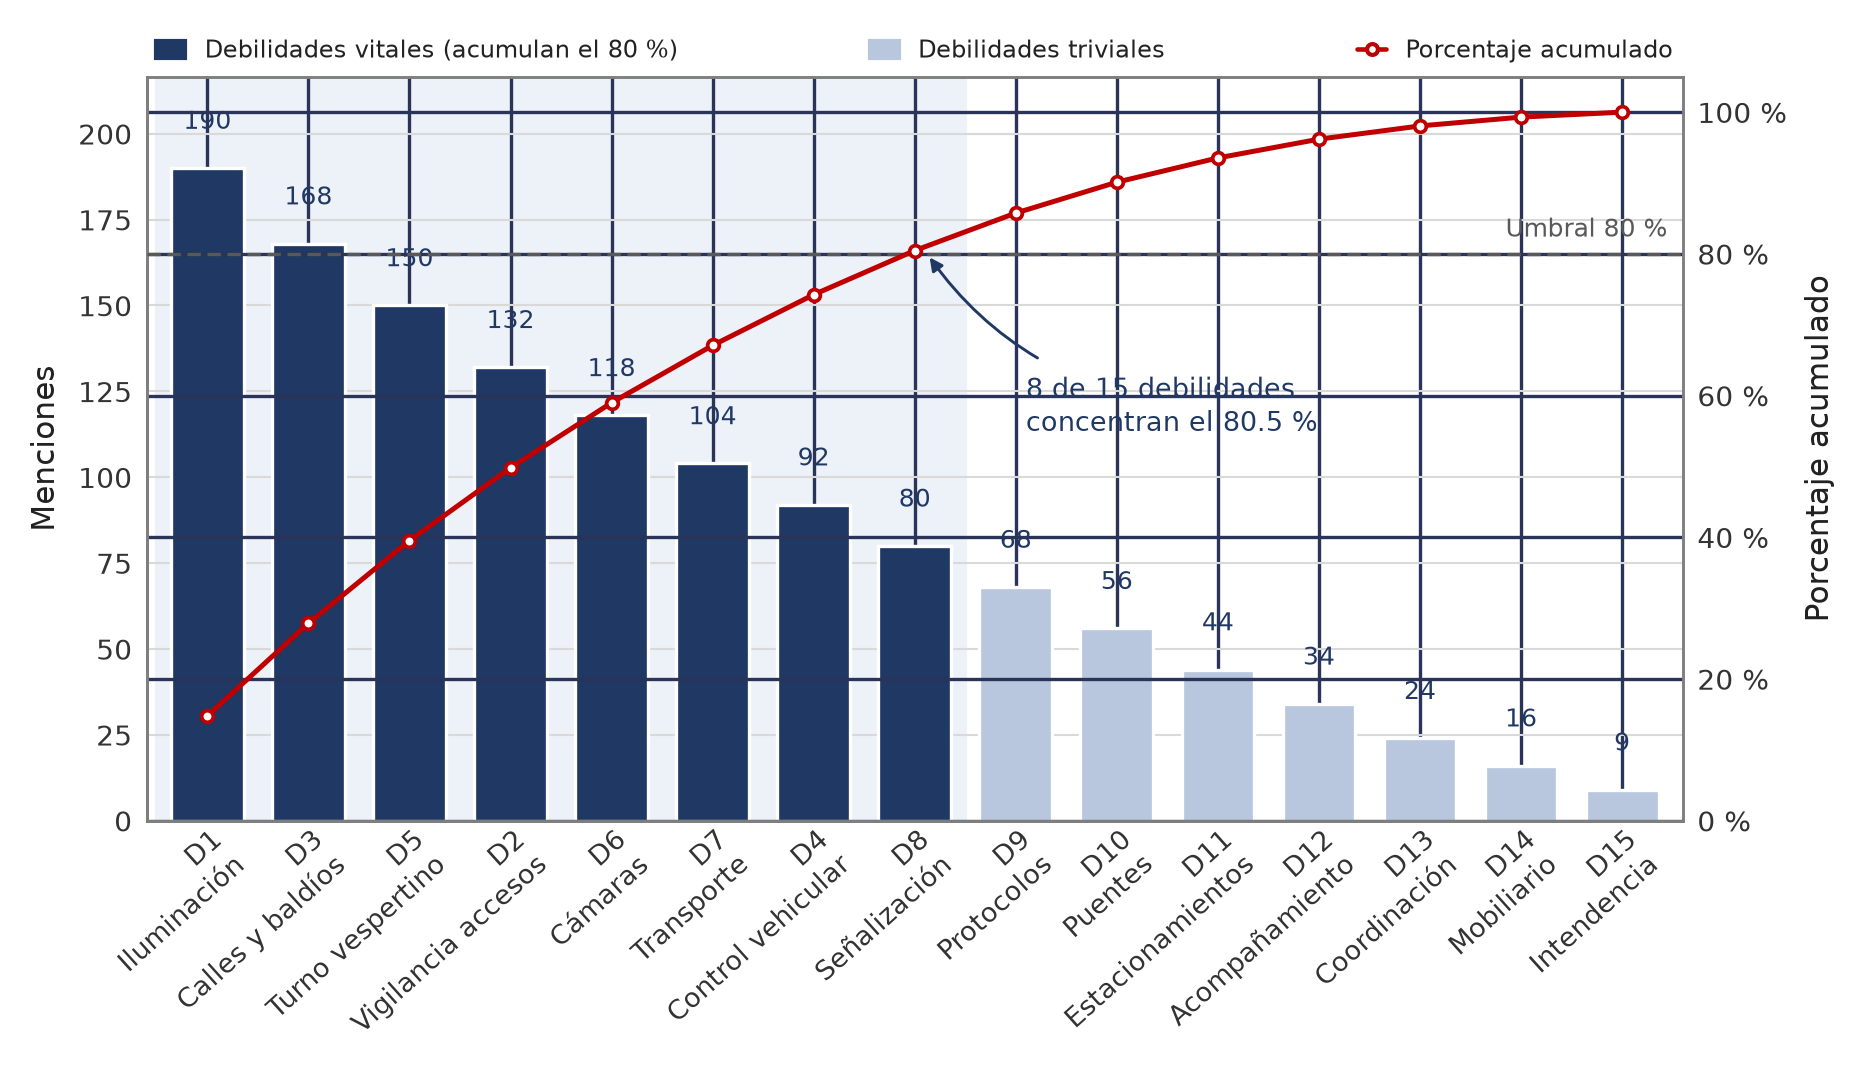
\includegraphics[width=\linewidth]{figuras/pareto.png}
  \caption{Diagrama de Pareto de las debilidades percibidas por los alumnos del
  Campus Siglo XXI. Ocho de las quince debilidades concentran el 80.47\,\% de
  las menciones.}
  \label{fig:pareto}
  \vspace{-2pt}
  {\footnotesize Fuente: elaboración propia y archivo \texttt{pareto.xlsx}.}
\end{figure}

\subsection{Lectura del diagrama}

El diagrama muestra tres hechos que conviene separar.

Primero, \textbf{la curva cae muy rápido al principio}. La debilidad más
mencionada, la iluminación, concentra por sí sola el 14.79\,\% de las menciones;
las tres primeras (iluminación, calles y turno vespertino) suman el 39.53\,\%.
No se trata de un problema difuso: hay un puñado de causas que explican una
parte desproporcionada del malestar.

Segundo, \textbf{el corte del 80\,\% cae en la octava debilidad}. Ocho de
quince planteamientos (53.3\,\% de las causas) acumulan el 80.47\,\% de las
menciones. Las siete restantes, que son casi la mitad de la lista, apenas
aportan el 19.53\,\%. Si la Universidad repartiera su esfuerzo por igual entre
las quince, dedicaría la mitad del trabajo a resolver una quinta parte del
problema.

Tercero, \textbf{las debilidades vitales comparten una naturaleza}. Seis de las
ocho primeras (D1, D2, D3, D5, D6 y D8) son condiciones del entorno físico y de
la operación cotidiana: luz, vigilancia, banquetas, horarios, cámaras y
señalización. De ellas, cinco puede modificar la Universidad con mantenimiento,
reasignación de personal o señalización (D1, D2, D5, D6 y D8); D4 exige una
inversión menor, y D3 y D7 dependen de convenios con el municipio y con los
transportistas. La mayor parte, aun así, se puede atender con medidas de bajo
costo y de efecto rápido.

\subsection{¿Por qué se concentra así?}

El patrón del Pareto no es casual. Detrás de la curva hay cuatro causas
estructurales que explican por qué unas debilidades se perciben mucho más que
otras.

\begin{enumerate}
  \item \textbf{El campus se diseñó hacia adentro.} La inversión en
        infraestructura se concentró en edificios, aulas y corredores, que son
        los espacios que se recorren todos los días y que se ven en los
        recorridos oficiales. El perímetro, los estacionamientos y los accesos
        peatonales quedaron como espacios residuales, sin un proyecto de
        iluminación ni de vegetación. La consecuencia es que el alumno percibe
        una diferencia brusca entre el interior iluminado y el exterior oscuro,
        y esa diferencia se registra como inseguridad.

  \item \textbf{La seguridad se contrató por turnos, no por riesgos.} El
        personal de vigilancia cubre el horario administrativo, de 7:00 a 19:00
        h, mientras que la salida del turno vespertino ocurre entre las 20:00 y
        las 21:30 h. El resultado es una paradoja: la hora de mayor afluencia y
        de mayor oscuridad es la que tiene menos personal. La percepción de los
        alumnos lo refleja con claridad: el 85.4\,\% de los encuestados del
        turno vespertino marcó D5, frente al 42.2\,\% del matutino.

  \item \textbf{El límite jurídico del campus detiene la gestión.} La
        Universidad es responsable de lo que ocurre dentro de su predio, pero
        la banqueta, la calle, el alumbrado y la parada son responsabilidad del
        municipio. Esa frontera produce un vacío: cada instancia cuida su parte
        y nadie atiende la transición. Las debilidades D3, D7 y D10 ---las
        calles, el transporte y los puentes--- caen justo en ese límite y, por
        eso, se perciben como problemas sin dueño.

  \item \textbf{Lo cotidiano pesa más que lo excepcional.} La encuesta mide
        percepciones acumuladas durante dos meses. La iluminación, la banqueta y
        el camión se viven todos los días; un protocolo de emergencia o un
        puente peatonal se usan pocas veces. El orden del Pareto refleja, en
        parte, esa frecuencia de exposición: no es que los protocolos importen
        menos, es que se experimentan menos.
\end{enumerate}

Estas cuatro causas explican por qué la curva tiene la forma que tiene y, sobre
todo, por qué las soluciones deben ser distintas: las dos primeras se corrigen
con mantenimiento y horarios; la tercera exige convenios; la cuarta, comunicación
y señalización.

\subsection{Los muchos triviales}

Las siete debilidades que quedan después del corte (D9 a D15) suman el
19.53\,\% de las menciones. Eso no significa que sean irrelevantes: significa
que, con recursos limitados, no son el primer lugar donde conviene invertir.
Algunas son baratas y pueden resolverse de inmediato, como el programa de
acompañamiento (D12) o la difusión de los protocolos (D9); otras exigen
inversión municipal o de largo plazo, como los puentes peatonales (D10). La
recomendación es atenderlas en una segunda fase, con excepción de aquellas que
impliquen un riesgo grave aunque su frecuencia sea baja, que deben evaluarse con
una matriz de riesgos y no solo con el Pareto.

% ===========================================================================
\section{Justificación de las debilidades prioritarias}

Esta sección explica, una por una, por qué las ocho debilidades vitales se
presentan en el campus. Cada explicación combina el dato de la encuesta con la
observación de campo y con una fuente documental. El orden es el del diagrama.

\subsection{D1. Iluminación insuficiente (190 menciones; 14.79\,\%)}

Es la debilidad más mencionada: la marcaron 190 de los 250 alumnos, es decir, el
76.0\,\% de la muestra. La percepción es más intensa en el turno vespertino
(84.5\,\%) que en el matutino (70.1\,\%), lo que tiene sentido: quien sale de
noche depende de la luz artificial para orientarse y para ser visto.

La literatura sobre prevención situacional es consistente en este punto. La
revisión sistemática de Welsh y Farrington encontró que la mejora del alumbrado
público reduce la delincuencia en las zonas intervenidas en alrededor de una
quinta parte \cite{welsh2008}. El mecanismo no es mágico: la luz aumenta la
vigilancia natural ---los vecinos, los guardias y los propios estudiantes ven
mejor--- y disuade a quien busca un punto ciego. Esa es también la lógica del
espacio defendible de Newman \cite{newman1972}.

En el campus, la observación de campo encontró tres problemas concretos. El
proyecto de luminarias LED cubrió el corredor central y la fachada, pero no el
perímetro ni el estacionamiento posterior; en un recorrido nocturno se contaron
nueve luminarias apagadas o intermitentes de un total de treinta y ocho; y la
vegetación de dos jardineras cubre parte de las luminarias del acceso sur. La
ENSU refuerza la relevancia del factor: el 55.9\,\% de la población urbana
señala el alumbrado público insuficiente como uno de los principales problemas
de su ciudad \cite{inegi2026ensu}. No es un detalle estético: es una condición
de seguridad.

\subsection{D3. Calles, banquetas y baldíos (168 menciones; 13.07\,\%)}

La segunda debilidad es el entorno inmediato. El 67.2\,\% de los alumnos la
marcó. Las banquetas de las calles laterales están rotas o invadidas por
puestos, la poda de los árboles se hace por temporada y no por visibilidad, y
hay lotes baldíos sin cerco que funcionan como atajos y como escondites.

La ENSU reporta que el 83.1\,\% de la población considera los baches en calles y
avenidas como uno de los principales problemas de su ciudad, y el 38.9\,\% los
parques y jardines descuidados \cite{inegi2026ensu}. El dato importa porque
muestra que el deterioro del espacio público no es una percepción exclusiva de
los estudiantes: es un problema urbano general que, en el campus, se vuelve
crítico porque obliga al peatón a caminar sobre la carpeta asfáltica.

Desde la criminología ambiental, un lote baldío hace tres cosas: elimina la
vigilancia natural, ofrece una ruta de escape y envía la señal de que nadie
cuida ese lugar \cite{newman1972, unodc2010}. La solución no es solo municipal:
la Universidad puede cercar y limpiar los predios que le pertenecen, y puede
negociar con los propietarios privados un convenio de mantenimiento.

\subsection{D5. Seguridad en el turno vespertino (150 menciones; 11.67\,\%)}

El 60.0\,\% de la muestra marcó esta debilidad, pero la cifra esconde una
brecha: la marcó el 85.4\,\% de los alumnos del vespertino y solo el 42.2\,\% de
los del matutino. La diferencia de 43 puntos porcentuales es la más grande de
todo el estudio y confirma que el problema es de horario, no de toda la jornada.

La ENSU aporta dos datos que ayudan a interpretarlo. El 35.8\,\% de la población
urbana cambió su hábito de caminar de noche en los alrededores de su vivienda
por temor al delito, y el 64.2\,\% de las mujeres se siente insegura en su
ciudad, frente al 50.6\,\% de los hombres \cite{inegi2026ensu}. En Zacatecas,
en noviembre, el sol se oculta antes de las 18:30 h; las clases del vespertino
terminan entre las 20:00 y las 21:30 h, y el turno de vigilancia concluye a las
19:00 h. La hora de salida queda, literalmente, fuera del horario de cobertura.

La causa es administrativa: el contrato de seguridad se diseñó para el horario
de oficina y no se ajustó cuando creció la matrícula del turno vespertino. La
consecuencia también es administrativa: se puede corregir con un cambio de
turnos, sin comprar equipo nuevo.

\subsection{D2. Vigilancia en accesos peatonales (132 menciones; 10.27\,\%)}

El 52.8\,\% de los alumnos percibe que los accesos peatonales no tienen
vigilancia suficiente. El campus tiene cinco accesos peatonales: en el turno
vespertino, cuatro cuentan con un guardia y el acceso principal con dos. En la
práctica, el guardia atiende al mismo tiempo el flujo de personas, el portón
vehicular y el monitoreo de las cámaras, lo que reduce su capacidad de
observación.

La guía de las Naciones Unidas sobre prevención del delito insiste en que la
vigilancia no depende solo del número de guardias, sino de su ubicación y de su
capacidad de ver sin obstáculos \cite{unodc2010}. Un guardia dentro de una
caseta no vigila la banqueta; un guardia en la banqueta, sí. La solución es
redistribuir, no necesariamente contratar: mover un puesto a la hora de mayor
flujo y establecer rondas cortas en los accesos laterales.

\subsection{D6. Puntos ciegos de las cámaras (118 menciones; 9.18\,\%)}

El 47.2\,\% de los alumnos señaló que las cámaras no cubren los lugares por
donde camina. La revisión de la instalación encontró 24 equipos, de los cuales 18
estaban operando; nueve no tenían visión nocturna y el almacenamiento era de
siete días. El perímetro posterior y el pasillo entre los edificios B y C
quedaban fuera del campo de visión.

Las cámaras no sustituyen a la vigilancia, pero sí disuaden y permiten
investigar. Su eficacia depende de tres condiciones: cobertura, grabación y
monitoreo. Si falla una, el equipo se vuelve un símbolo. La ENSU reporta que, entre quienes
atestiguaron conductas delictivas en los alrededores de su vivienda, el
45.3\,\% mencionó robos o asaltos \cite{inegi2026ensu}; en un entorno con esa
frecuencia, la cobertura del perímetro debería ser la prioridad de la inversión
en tecnología.

\subsection{D7. Transporte y paradas (104 menciones; 8.09\,\%)}

El 41.6\,\% de los alumnos marcó esta debilidad; en el vespertino sube al
49.5\,\%. La parada más cercana está a unos 400 metros del acceso principal, no
tiene techo ni iluminación propia, y la última corrida pasa alrededor de las
21:00 h. Quien pierde el camión debe esperar en la avenida o caminar hasta la
siguiente parada.

La ENSU reporta que el 61.1\,\% de la población se siente insegura en el
transporte público y el 37.9\,\% califica el servicio como deficiente
\cite{inegi2026ensu}. El estudio de Hernández Romero sobre estudiantes
universitarios del Estado de México encontró el mismo patrón: la inseguridad se
concentra en la espera y en el trayecto, y los alumnos modifican horarios y
rutas para evitarla \cite{hernandez2021}. La solución tiene dos partes: una
parada segura dentro del campus, con luz y vigilancia, y un convenio con los
concesionarios para garantizar corridas después de las 21:00 h.

\subsection{D4. Control de acceso vehicular (92 menciones; 7.16\,\%)}

El 36.8\,\% de los alumnos percibe que cualquier vehículo puede entrar. La
caseta registra a los visitantes de manera informal, no pide credencial a los
conductores y no tiene pluma ni control de placas. El acceso se diseñó para la
fluidez, no para la seguridad, y esa prioridad se mantiene aunque el campus haya
crecido.

El control de acceso es una de las medidas más antiguas de la prevención
situacional: aumentar el esfuerzo percibido por el delincuente y reducir su
anonimato \cite{unodc2010}. No requiere tecnología costosa: una credencial
visible, un registro de visitantes y una pluma manual resuelven la mayor parte
del problema. El robo de autopartes y el ingreso de vehículos ajenos son los
delitos que esta medida previene.

\subsection{D8. Señalización y rutas seguras (80 menciones; 6.23\,\%)}

El 32.0\,\% de los alumnos no sabe cuál es la ruta más segura para salir ni a
dónde llamar en una emergencia. La señalización existente es escasa y está
desactualizada; los números de emergencia se difunden por redes sociales, pero
no están en los pasillos ni en los accesos.

La señalización cumple dos funciones: orienta y tranquiliza. Un mapa de rutas
seguras, con los puntos de luz, las casetas y los teléfonos, reduce la
incertidumbre y ayuda a que el alumno tome decisiones con información. Es una de
las medidas más baratas del plan y una de las que más rápido se perciben. Por
eso, aunque su frecuencia es menor que la de D1 o D3, su relación costo--efecto
es alta.

\subsection{Las siete debilidades restantes}

Las debilidades D9 a D15 concentran el 19.53\,\% de las menciones. Los
protocolos de emergencia (D9, 68 menciones) fallan por difusión, no por diseño:
existen, pero el alumno no los conoce. Los puentes y pasos a desnivel (D10, 56)
dependen del municipio y requieren inversión de largo plazo. Los estacionamientos
(D11, 44) y el mobiliario (D14, 16) son problemas de mantenimiento. El
acompañamiento (D12, 34), la coordinación policial (D13, 24) y la intendencia
(D15, 9) son los de menor frecuencia, aunque el acompañamiento tiene un costo
casi nulo y un efecto inmediato en la percepción.

La conclusión de este bloque es la misma que la del Pareto: no se trata de
ignorar estas debilidades, sino de no empezar por ellas. Un plan que atienda
primero las ocho vitales y después las siete restantes obtiene más resultados
con el mismo presupuesto.

% ===========================================================================
\section{Plan de atención}

A partir del Pareto se propone un plan de ocho acciones, una por cada debilidad
vital. El criterio de prioridad es el orden del diagrama; el plazo es el tiempo
máximo para la primera evidencia; el indicador permite verificar el avance sin
depender de impresiones.

\begin{table}[H]
\centering
\footnotesize
\caption{Plan de atención de las debilidades vitales.}
\label{tab:plan}
\begin{tabularx}{\linewidth}{@{}L{1.15cm}L{3.0cm}L{5.6cm}L{3.25cm}L{1.3cm}@{}}
\toprule
\textbf{Prior.} & \textbf{Debilidad} & \textbf{Acción} & \textbf{Indicador} & \textbf{Plazo} \\
\midrule
1 & D1 Iluminación &
    Censo de luminarias, sustitución de las fundidas y poda que despeje las
    luminarias del perímetro; recorrido nocturno mensual. &
    Porcentaje de luminarias funcionales (meta: 98\,\%). & 30 días \\
2 & D5 Turno vespertino &
    Reasignar dos guardias al cierre del vespertino (19:00--21:30 h) y
    establecer rondas en los accesos. &
    Guardias por acceso en hora pico (meta: 2). & 15 días \\
3 & D3 Calles y baldíos &
    Convenio con el municipio para poda, bacheo y limpieza de baldíos; cerco
    de los predios universitarios. &
    Metros de banqueta rehabilitados; lotes cercados. & 90 días \\
4 & D2 Accesos peatonales &
    Redistribuir puestos, colocar una silla y una mesa de registro en cada
    acceso lateral. &
    Cobertura de los cinco accesos en hora pico. & 30 días \\
5 & D6 Cámaras &
    Auditoría de cobertura, reubicación de seis equipos y ampliación del
    almacenamiento a 30 días. &
    Porcentaje del perímetro cubierto (meta: 90\,\%). & 60 días \\
6 & D7 Transporte &
    Habilitar una parada segura dentro del campus y convenir corridas
    posteriores a las 21:00 h. &
    Tiempo de espera promedio (meta: 10 min). & 60 días \\
7 & D4 Acceso vehicular &
    Credencial visible, registro de visitantes y pluma de control en la
    caseta principal. &
    Porcentaje de vehículos registrados (meta: 100\,\%). & 45 días \\
8 & D8 Señalización &
    Mapa de rutas seguras en cada acceso, señalética de emergencia y
    directorio visible. &
    Accesos con mapa y directorio (meta: 5 de 5). & 30 días \\
\bottomrule
\end{tabularx}
\end{table}

El plan sigue el ciclo de mejora continua \cite{deming1989}. En la etapa de
\emph{planeación} se ejecutan las acciones de bajo costo (D5, D2, D8), que no
requieren compra de equipo; en la de \emph{hacer}, se aplican las de
mantenimiento y convenio (D1, D3, D4); en la de \emph{verificar}, se vuelve a
aplicar la encuesta al final del semestre y se compara el nuevo Pareto con el de
la figura~\ref{fig:pareto}; en la de \emph{actuar}, se ajustan las acciones que
no movieron el indicador y se incorporan las debilidades que hayan subido de
lugar. El libro de Excel sirve como tablero: al actualizar las marcas, la tabla y
el gráfico se recalculan solos.

% ===========================================================================
\section{Conclusiones}

El análisis permitió responder la pregunta inicial. De las quince debilidades
del FODA, ocho concentran el 80.47\,\% de las menciones: iluminación, calles y
baldíos, seguridad en el turno vespertino, vigilancia en los accesos, puntos
ciegos de las cámaras, transporte y paradas, control vehicular y señalización.
Las siete restantes, que son casi la mitad de la lista, explican apenas una
quinta parte del problema. Esa es la aportación práctica del Pareto: convierte
una lista de quince preocupaciones en un orden de trabajo.

El FODA mostró que el campus tiene más recursos de los que parece. La comunidad
organizada, la videovigilancia, el personal de seguridad y el procedimiento de
reporte existen y pueden reorientarse sin inversión nueva. El problema no es la
falta de infraestructura, sino su distribución: el interior del campus está
atendido y el perímetro no. Las debilidades vitales comparten esa ubicación y
esa lógica, lo que explica por qué la curva del Pareto es tan pronunciada.

La justificación documental confirmó que el fenómeno no es exclusivo del
campus. La ENSU reporta una percepción de inseguridad de 77.3\,\% en el área
urbana de Zacatecas, muy por encima del promedio nacional, y muestra que la
calle, el transporte y el alumbrado son los espacios y factores que más pesan en
esa percepción \cite{inegi2026ensu}. La literatura sobre alumbrado, vigilancia
natural y prevención situacional explica el mecanismo: el entorno no determina
la conducta, pero sí cambia el costo y la oportunidad del delito
\cite{welsh2008, newman1972, unodc2010}.

El trabajo tiene limitaciones que deben declararse. La muestra es no
probabilística y de un solo campus; la frecuencia no mide gravedad; y la base de
este ejercicio se construyó por simulación calibrada, como se explicó en el
apartado 4.5. Para una siguiente etapa se recomienda aplicar el instrumento a
una muestra probabilística, incorporar una matriz de riesgos que pondere la
gravedad y repetir la medición al final del semestre para verificar el efecto de
las acciones.

Aun con esas limitaciones, la conclusión de fondo se sostiene: la inseguridad
en los horarios de entrada y salida no se combate con una medida aislada, sino
con una cartera de medidas priorizadas, medibles y evaluables. El diagrama de
Pareto no resuelve el problema, pero dice por dónde empezar; y en un tema donde
los recursos siempre son menores que las necesidades, saber por dónde empezar es
la mitad del trabajo.

% ===========================================================================
\addcontentsline{toc}{section}{Bibliografía}

\begin{thebibliography}{15}
\footnotesize
\setlength{\itemsep}{2pt}
\setlength{\parskip}{0pt}

\bibitem{inegi2026ensu}
INEGI, \textit{Encuesta Nacional de Seguridad Pública Urbana (ENSU). Tercer
trimestre de 2026. Reporte de resultados 49/26}. Aguascalientes: Instituto
Nacional de Estadística y Geografía, 23 de octubre de 2026.
\url{https://www.inegi.org.mx/programas/ensu/}

\bibitem{sesnsp2026}
Secretariado Ejecutivo del Sistema Nacional de Seguridad Pública,
\textit{Incidencia delictiva del fuero común, nueva metodología}. Ciudad de
México: SESNSP, 2026.
\url{https://www.gob.mx/sesnsp/acciones-y-programas/incidencia-delictiva-del-fuero-comun-nueva-metodologia}

\bibitem{hernandez2021}
M. Hernández Romero, ``Percepción de inseguridad en el transporte público: el
caso de los estudiantes universitarios del CU UAEM Zumpango, en el Estado de
México'', \textit{Collectivus, Revista de Ciencias Sociales}, vol. 8, núm. 1,
2021. doi: 10.15648/collectivus.vol8num1.2021.2954

\bibitem{welsh2008}
B. C. Welsh y D. P. Farrington, ``Effects of Improved Street Lighting on
Crime'', \textit{Campbell Systematic Reviews}, vol. 4, núm. 1, 2008.
doi: 10.4073/csr.2008.13

\bibitem{newman1972}
O. Newman, \textit{Defensible Space: Crime Prevention Through Urban Design}.
Nueva York: Macmillan, 1972.

\bibitem{unodc2010}
Oficina de las Naciones Unidas contra la Droga y el Delito, \textit{Handbook on
the Crime Prevention Guidelines: Making them Work}. Viena: Naciones Unidas,
2010.

\bibitem{juran2015}
J. M. Juran y J. A. De Feo, \textit{Juran's Quality Handbook: The Official Guide
to the Standard Approach to Quality}, 7.ª ed. Nueva York: McGraw-Hill, 2015.

\bibitem{ishikawa1986}
K. Ishikawa, \textit{Guide to Quality Control}, 2.ª ed. Tokio: Asian
Productivity Organization, 1986.

\bibitem{gutierrez2014}
H. Gutiérrez Pulido, \textit{Calidad total y productividad}, 4.ª ed. México:
McGraw-Hill, 2014.

\bibitem{deming1989}
W. E. Deming, \textit{Out of the Crisis}. Cambridge, MA: MIT Press, 1989.

\bibitem{weihrich1982}
H. Weihrich, ``The TOWS Matrix: A Tool for Situational Analysis'', \textit{Long
Range Planning}, vol. 15, núm. 2, pp. 54--66, 1982.
doi: 10.1016/0024-6301(82)90120-0

\bibitem{pareto1896}
V. Pareto, \textit{Cours d'économie politique}. Lausana: F. Rouge, 1896.

\bibitem{cpeum}
Cámara de Diputados del H. Congreso de la Unión, \textit{Constitución Política
de los Estados Unidos Mexicanos}, artículo 3.º. México, texto vigente 2026.

\bibitem{lges2021}
Cámara de Diputados del H. Congreso de la Unión, \textit{Ley General de
Educación Superior}. México: Diario Oficial de la Federación, 20 de abril de
2021.

\end{thebibliography}

% ===========================================================================
\appendix
\section{Cuestionario aplicado}

\begin{table}[H]
\centering
\small
\caption{Reactivos del cuestionario (respuesta múltiple).}
\label{tab:cuestionario}
\begin{tabularx}{\linewidth}{@{}clX@{}}
\toprule
\textbf{Núm.} & \textbf{Clave} & \textbf{En tus entradas o salidas del campus, ¿has percibido\ldots?} \\
\midrule
1  & D1  & Iluminación insuficiente en accesos, andadores o estacionamientos. \\
2  & D2  & Falta de vigilancia en los accesos peatonales en horas pico. \\
3  & D3  & Calles aledañas con banquetas rotas, poda excesiva o lotes baldíos. \\
4  & D4  & Falta de control del acceso vehicular o de identificación de conductores. \\
5  & D5  & Poca presencia de seguridad al salir del turno vespertino. \\
6  & D6  & Cámaras mal ubicadas o fuera de servicio que dejan puntos ciegos. \\
7  & D7  & Transporte público insuficiente o paradas alejadas y sin iluminación. \\
8  & D8  & Falta de señalización o de rutas peatonales seguras. \\
9  & D9  & Desconocimiento de los protocolos y números de emergencia. \\
10 & D10 & Puentes peatonales o pasos a desnivel inexistentes o en mal estado. \\
11 & D11 & Estacionamientos sin delimitación, numeración o control. \\
12 & D12 & Ausencia de programas de acompañamiento entre alumnos. \\
13 & D13 & Coordinación débil con la policía municipal o estatal. \\
14 & D14 & Mobiliario urbano vandalizado o sin mantenimiento. \\
15 & D15 & Falta de intendencia o vigilancia en los últimos minutos de la jornada. \\
\bottomrule
\end{tabularx}
\end{table}

\noindent\textbf{Datos generales:} sexo (M/F), turno (matutino/vespertino),
semestre (1, 3, 5, 7 o 9) y área académica (Ciencias de la Salud, Ingeniería, Ciencias
Básicas o Posgrado).

\noindent\textbf{Instrucción:} marque todas las situaciones que haya percibido
en los últimos dos meses. No hay respuestas correctas ni incorrectas.

% ===========================================================================
\section{Datos por turno}

La tabla~\ref{tab:turno} presenta las tres debilidades en las que la diferencia
entre turnos resultó más clara. Es la evidencia que sustenta la interpretación
del apartado 7.3: la salida del vespertino ocurre de noche y con menos
cobertura.

\begin{table}[H]
\centering
\small
\caption{Porcentaje de alumnos que marcó cada debilidad, según el turno.}
\label{tab:turno}
\begin{tabular}{@{}lrrr@{}}
\toprule
\textbf{Debilidad} & \textbf{Matutino} & \textbf{Vespertino} & \textbf{Diferencia} \\
 & \textbf{($n=147$)} & \textbf{($n=103$)} & \\
\midrule
D1. Iluminación & 70.1\,\% & 84.5\,\% & +14.4 \\
D5. Seguridad al salir & 42.2\,\% & 85.4\,\% & +43.2 \\
D7. Transporte y paradas & 36.1\,\% & 49.5\,\% & +13.4 \\
\bottomrule
\end{tabular}

\vspace{4pt}
\begin{minipage}{0.9\linewidth}
\footnotesize
Fuente: elaboración propia con los microdatos de la encuesta. El turno matutino
representa el 58.8\,\% de la muestra y el vespertino el 41.2\,\%.
\end{minipage}
\end{table}

\end{document}
